\section{Resultados}

\subsection{Modulação AM-DSB-SC (Double Sideband Suppressed Carrier)}

Na modulação AM-DSB-SC, espera-se observar o espectro da mensagem deslocado para as frequências laterais em torno da frequência da portadora, conforme ilustrado na Figura~\ref{fig:sinais_freq_am_dsb}. Como pode ser visualizado, a mensagem original, que é uma senoide de 1~kHz, aparece como dois impulsos simétricos em torno da portadora de 5~kHz, definida pelo QT GUI Range. Isso ocorre devido à propriedade da modulação, que desloca o espectro da mensagem para as frequências $f_c + f_m$ e $f_c - f_m$, onde $f_c$ é a frequência da portadora e $f_m$ a frequência da mensagem.

\begin{figure}[h]
    \centering
    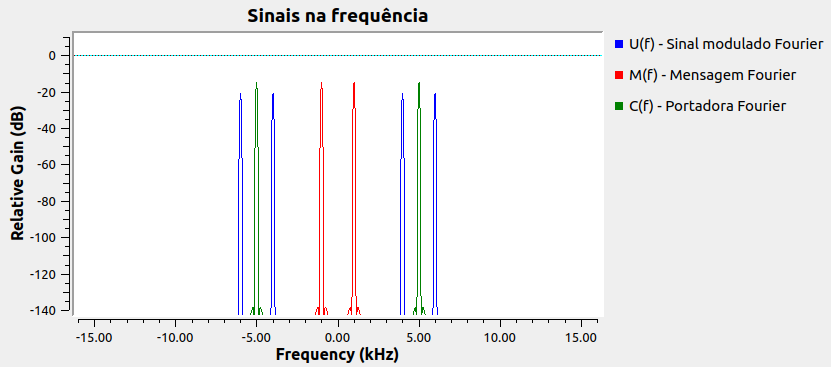
\includegraphics[width=0.5\textwidth]{images/sinais_freqe_gnu.png}
    \caption{Sinais no domínio da frequência. Fonte: Autor.}
    \label{fig:sinais_freq_am_dsb}
\end{figure}

\subsection{Demodulação AM-DSB-SC (Double Sideband Suppressed Carrier)}

Os resultados da demodulação também estão de acordo com o esperado. Ao utilizar um filtro passa-baixa com frequência de corte superior à largura de banda da mensagem, é possível recuperar o sinal original. A Figura~\ref{fig:demodulacao_am_dsb} mostra o espectro do sinal após a demodulação, evidenciando a recuperação da senoide de 1~kHz.

\begin{figure}[h]
    \centering
    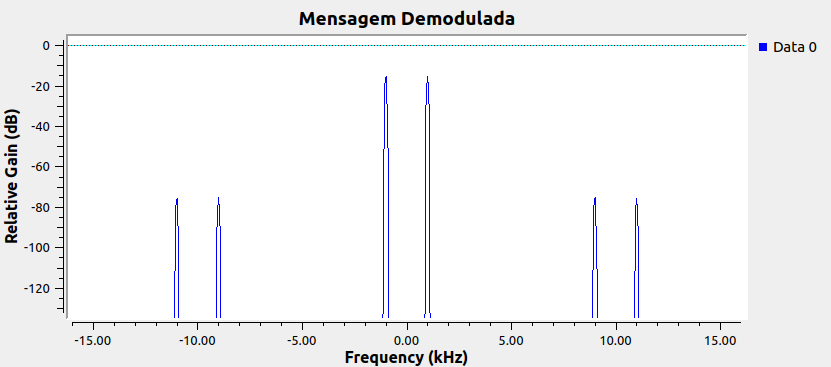
\includegraphics[width=0.5\textwidth]{images/demodulacao_am_dsb_freq.png}
    \caption{Demodulação do sinal AM-DSB-SC. Fonte: Autor.}
    \label{fig:demodulacao_am_dsb}
\end{figure}

\subsection{Falta de Sincronismo}

Para demonstrar que a demodulação AM-DSB-SC exige sincronismo entre a portadora do transmissor e do receptor, foi alterada a frequência da portadora local no receptor para 10~kHz utilizando o QT GUI Range, simulando uma perda de sincronismo de frequência. A Figura~\ref{fig:falta_sincronismo_dsb} mostra o espectro do sinal demodulado sob essa condição, evidenciando distorções e a impossibilidade de recuperar corretamente a mensagem original.

\begin{figure}[h]
    \centering
    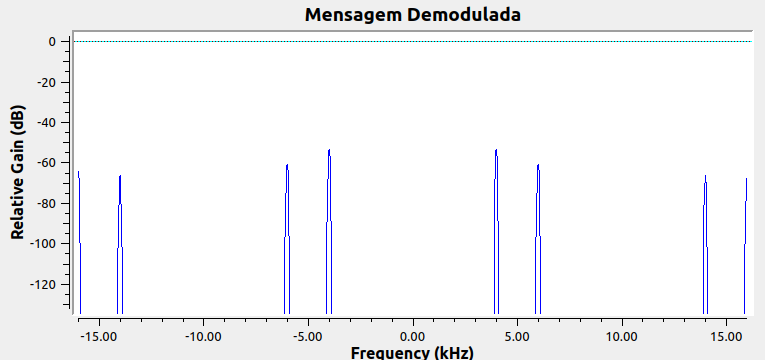
\includegraphics[width=0.5\textwidth]{images/falta_sincronismo_dsb.png}
    \caption{Simulação de falta de sincronismo na demodulação AM-DSB-SC. Fonte: Autor.}
    \label{fig:falta_sincronismo_dsb}
\end{figure}



